\documentclass[tikz,border=10pt]{standalone}
\usepackage{amsmath,amssymb}
\usetikzlibrary{arrows.meta,positioning,calc}

\definecolor{edgecol}{RGB}{110,100,200}
\definecolor{nodecol}{RGB}{40,40,160}
\definecolor{topicc}{RGB}{210,90,20}   % topic embedding (row of V)
\definecolor{userc}{RGB}{0,130,90}     % positive user
\definecolor{negc}{RGB}{180,40,40}     % negative users

\tikzset{
  neuron/.style={circle, draw=nodecol, thick, minimum size=0.95cm, inner sep=0pt, font=\small},
  active/.style={neuron, draw=topicc, fill=topicc!15},
  skipped/.style={neuron, draw=black!35, dashed, text=black!40},
  lbl/.style={font=\bfseries\small, text=black!70, align=center},
  conn/.style={edgecol!40, line width=0.3pt},
  elab/.style={fill=white, inner sep=1pt, font=\scriptsize},
}

\begin{document}
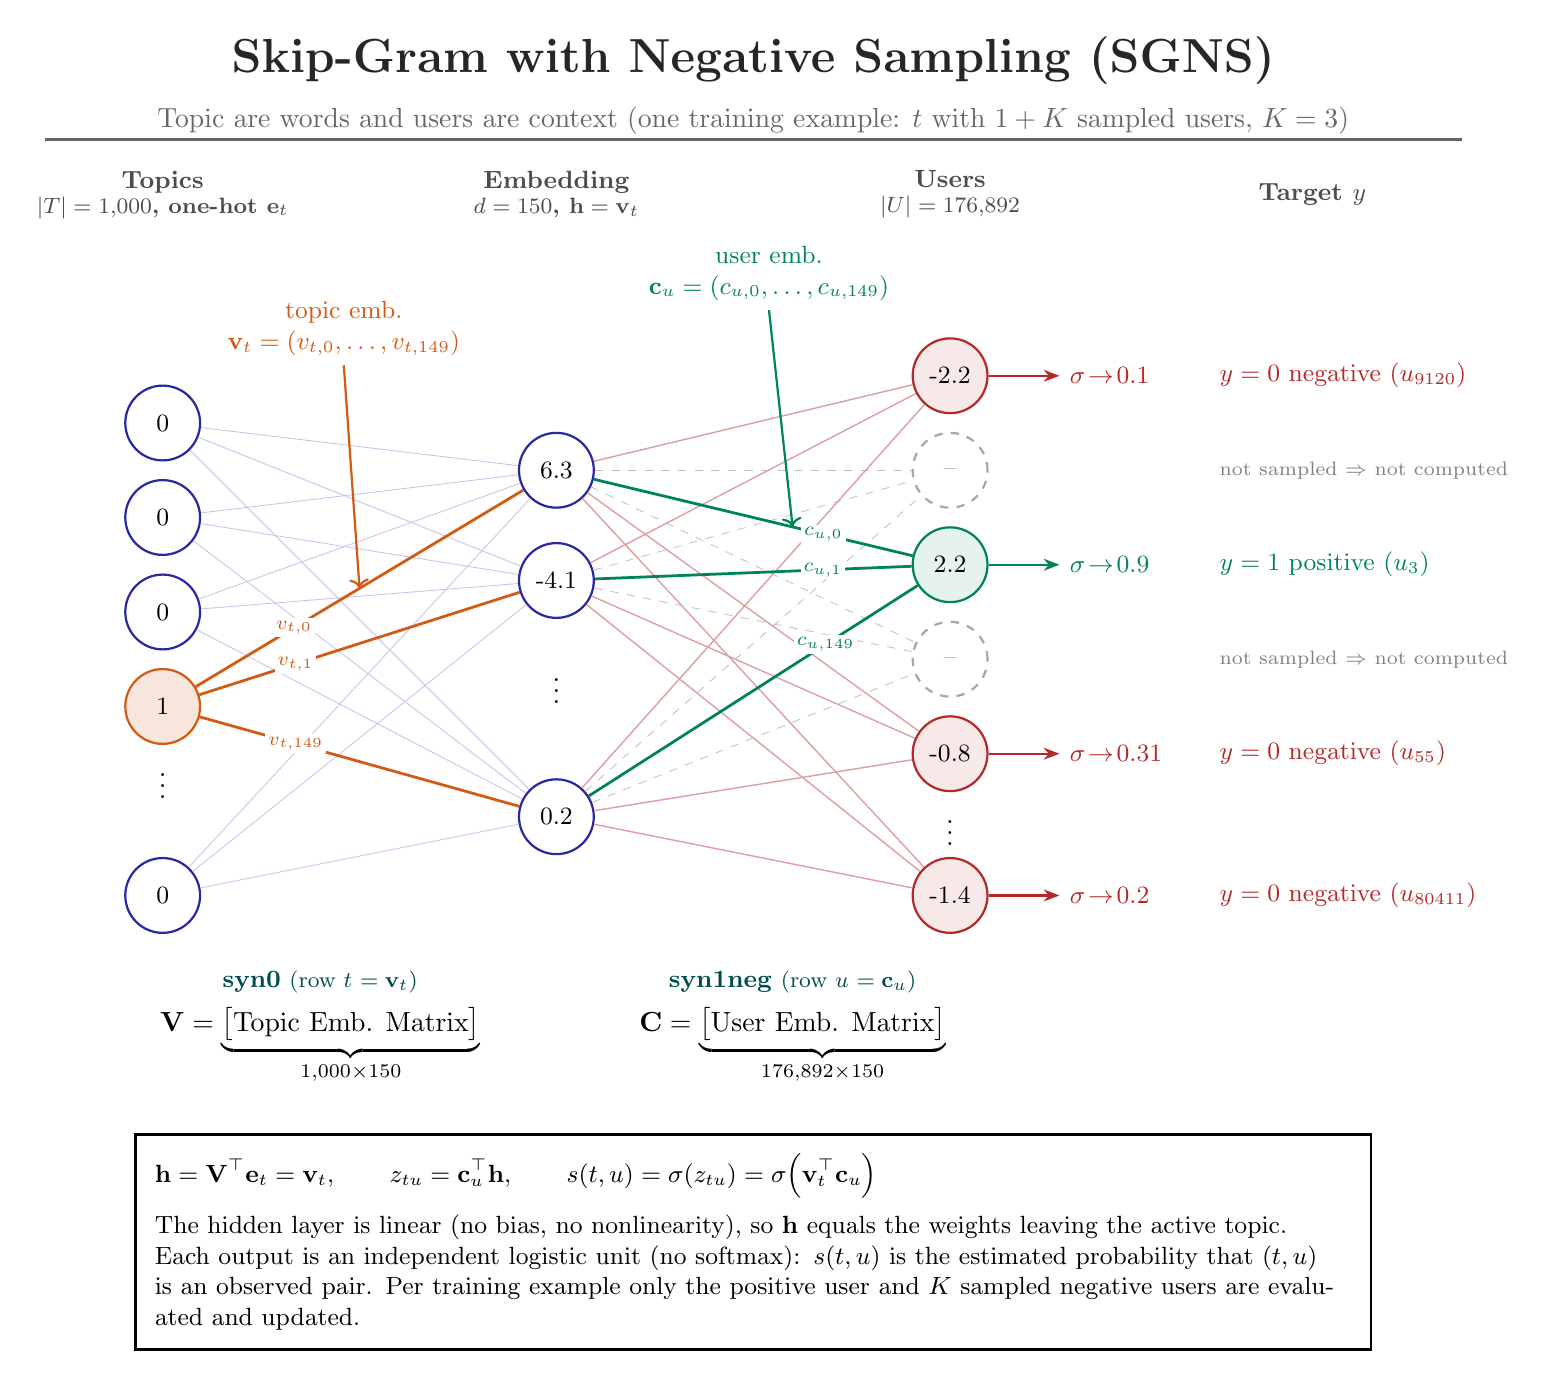
\begin{tikzpicture}

% ---------- Title ----------
\node[font=\LARGE\bfseries, text=black!85] (title) at (7.5,7.6)
  {Skip-Gram with Negative Sampling (SGNS)};
\node[font=\normalsize, text=black!60, below=1pt of title]
  {Topic are words and users are context (one training example: $t$ with $1+K$ sampled users, $K=3$)};
\draw[black!60, line width=0.8pt] (-1.5,6.6) -- (16.5,6.6);

% ---------- Layer headers ----------
\node[lbl] at (0,5.9)    {Topics\\[-2pt]\footnotesize $|T|=1{,}000$, one-hot $\mathbf{e}_t$};
\node[lbl] at (5,5.9)    {Embedding\\[-2pt]\footnotesize $d=150$, $\mathbf{h}=\mathbf{v}_t$};
\node[lbl] at (10,5.9)   {Users\\[-2pt]\footnotesize $|U|=176{,}892$};
\node[lbl] at (14.6,5.9) {Target $y$};

% ---------- Input layer (one-hot topics) ----------
\node[neuron] (i1) at (0, 3.0) {0};
\node[neuron] (i2) at (0, 1.8) {0};
\node[neuron] (i3) at (0, 0.6) {0};
\node[active] (i4) at (0,-0.6) {1};
\node          at (0,-1.5) {$\vdots$};
\node[neuron] (i5) at (0,-3.0) {0};

% ---------- Hidden layer (h = v_t, linear, no bias) ----------
\node[neuron] (h1) at (5, 2.4) {6.3};
\node[neuron] (h2) at (5, 1.0) {-4.1};
\node          at (5,-0.3) {$\vdots$};
\node[neuron] (h3) at (5,-2.0) {0.2};

% ---------- Output layer ----------
% sampled users: z = c_u^T v_t, sigma(z), target y
\foreach \k/\y/\lg/\col/\tg/\txt in {
    1/3.6/-2.2/negc/0/{negative ($u_{9120}$)},
    3/1.2/2.2/userc/1/{positive ($u_{3}$)},
    5/-1.2/-0.8/negc/0/{negative ($u_{55}$)},
    6/-3.0/-1.4/negc/0/{negative ($u_{80411}$)}}{
  \node[neuron, draw=\col, fill=\col!10] (o\k) at (10,\y) {\lg};
  \pgfmathsetmacro\sv{1/(1+exp(-(\lg)))}
  \draw[-{Stealth[length=2mm]}, thick, \col] (o\k.east) -- ++(0.9,0)
      node[right, font=\small] {$\sigma\!\rightarrow\!\pgfmathprintnumber[fixed,precision=2]{\sv}$};
  \node[anchor=west, font=\small, text=\col] at (13.3,\y) {$y=\tg$\ \txt};
}
% users that were not sampled: nothing is computed for them
\node[skipped] (o2) at (10, 2.4) {--};
\node[skipped] (o4) at (10, 0.0) {--};
\foreach \y in {2.4,0.0}{
  \node[anchor=west, font=\scriptsize, text=black!50, align=left] at (13.3,\y)
      {not sampled $\Rightarrow$ not computed};
}
\node at (10,-2.1) {$\vdots$};

% ---------- Edges: input -> hidden ----------
\foreach \i in {i1,i2,i3,i5}{\foreach \h in {h1,h2,h3}{\draw[conn] (\i) -- (\h);}}
% weights leaving the active topic = topic embedding v_t (so that h_j = v_{t,j})
\draw[topicc, line width=1pt] (i4) -- (h1) node[pos=0.30, elab] {$v_{t,0}$};
\draw[topicc, line width=1pt] (i4) -- (h2) node[pos=0.30, elab] {$v_{t,1}$};
\draw[topicc, line width=1pt] (i4) -- (h3) node[pos=0.30, elab] {$v_{t,149}$};

% ---------- Edges: hidden -> output ----------
\foreach \h in {h1,h2,h3}{
  \foreach \oo in {o1,o5,o6}{\draw[negc!45, line width=0.5pt] (\h) -- (\oo);}
  \foreach \oo in {o2,o4}{\draw[black!25, dashed, line width=0.3pt] (\h) -- (\oo);}
}
% weights entering the positive user = user embedding c_u
\draw[userc, line width=1pt] (h1) -- (o3) node[pos=0.72, elab] {$c_{u,0}$};
\draw[userc, line width=1pt] (h2) -- (o3) node[pos=0.72, elab] {$c_{u,1}$};
\draw[userc, line width=1pt] (h3) -- (o3) node[pos=0.72, elab] {$c_{u,149}$};

% ---------- Embedding annotations ----------
\node[text=topicc, font=\small, align=center] (tann) at (2.3,4.2)
  {topic emb.\\ $\mathbf{v}_t=(v_{t,0},\dots,v_{t,149})$};
\draw[->, topicc, thick] (tann.south) -- ($(i4)!0.5!(h1)$);

\node[text=userc, font=\small, align=center] (uann) at (7.7,4.9)
  {user emb.\\ $\mathbf{c}_u=(c_{u,0},\dots,c_{u,149})$};
\draw[->, userc, thick] (uann.south) -- ($(h1)!0.6!(o3)$);

% ---------- Matrices ----------
\node[font=\small, text=teal!60!black] at (2.0,-4.1)
  {\textbf{syn0}\ \footnotesize (row $t$ $=\mathbf{v}_t$)};
\node[anchor=north] at (2.0,-4.3)
  {$\mathbf{V}=\underbrace{\big[\text{Topic Emb. Matrix}\big]}_{1{,}000\times150}$};

\node[font=\small, text=teal!60!black] at (8.0,-4.1)
  {\textbf{syn1neg}\ \footnotesize (row $u$ $=\mathbf{c}_u$)};
\node[anchor=north] at (8.0,-4.3)
  {$\mathbf{C}=\underbrace{\big[\text{User Emb. Matrix}\big]}_{176{,}892\times150}$};

% ---------- Forward pass ----------
\node[draw, thick, inner sep=7pt, align=left, text width=15.2cm, font=\small]
  at (7.5,-7.4)
  {$\displaystyle \mathbf{h}=\mathbf{V}^{\top}\mathbf{e}_t=\mathbf{v}_t,\qquad
     z_{tu}=\mathbf{c}_u^{\top}\mathbf{h},\qquad
     s(t,u)=\sigma(z_{tu})=\sigma\!\left(\mathbf{v}_t^{\top}\mathbf{c}_u\right)$\\[5pt]
   The hidden layer is linear (no bias, no nonlinearity), so $\mathbf{h}$ equals the weights leaving
   the active topic. Each output is an independent logistic unit (no softmax):
   $s(t,u)$ is the estimated probability that $(t,u)$ is an observed pair. Per training
   example only the positive user and $K$ sampled negative users are evaluated and updated.};

\end{tikzpicture}
\end{document}